\documentclass[11pt,a4paper,titlepage]{article}
\usepackage[a4paper]{geometry}
\usepackage[utf8]{inputenc}
\usepackage[english]{babel}
\usepackage{lipsum}

\usepackage{amsmath, amssymb, amsfonts, amsthm, mathtools, physics}
% mathtools for: Aboxed (put box on last equation in align envirenment)
\usepackage{microtype} %improves the spacing between words and letters
\usepackage{listings} %insert codeblocks
\usepackage{graphicx} %package to manage images
\usepackage{float} %force figure placement
\graphicspath{ {Code/} }



%%%%%%%%%%%%%%%%%%%%%%%%%%%%%%%%%%%%%%%%%%%%%%%%%%
%    SECTIONS
%%%%%%%%%%%%%%%%%%%%%%%%%%%%%%%%%%%%%%%%%%%%%%%%%%
\usepackage{titlesec}
\usepackage{sectsty}
%%%%%%%%%%%%%%%%%%%%%%%%
%set section enumerator to arabic number (see footnotes markings alternatives)
\renewcommand\thesection{Question \arabic{section}} %define sections numbering
\renewcommand\thesubsection{\arabic{section}.\alph{subsection}} %number.letter
\renewcommand\thesubsubsection{\arabic{section}.\alph{subsection}.\roman{subsubsection}} %tabbed roman numeral

%define new section style
\newcommand{\mysection}{
\titleformat{\section} [runin] {\usefont{OT1}{lmss}{b}{n}} 
{\thesection} {3pt} {} } 



%%%%%%%%%%%%%%%%%%%%%%%%%%%%%%%%%%%%%%%%%%%%%%%%%%
%		Shortcuts
%%%%%%%%%%%%%%%%%%%%%%%%%%%%%%%%%%%%%%%%%%%%%%%%%%
\newcommand{\R}{\mathbb{R}}



\makeatletter
\let\reftagform@=\tagform@
\def\tagform@#1{\maketag@@@{(\ignorespaces\textcolor{red}{#1}\unskip\@@italiccorr)}}
\renewcommand{\eqref}[1]{\textup{\reftagform@{\ref{#1}}}}
\makeatother
\usepackage{hyperref}
\hypersetup{colorlinks=true}

%%%%%%%%%%%%%%%%%%%%%%%%%%%%%%%%%%%%%%%%%%%%%%%%%%
%% PREPARE TITLE
%%%%%%%%%%%%%%%%%%%%%%%%%%%%%%%%%%%%%%%%%%%%%%%%%%
\title{CS 229: Machine Learning\\
Problem Set $1$}
\author{William Ma}
\date{\today}
%%%%%%%%%%%%%%%%%%%%%%%%%%%%%%%%%%%%%%%%%%%%%%%%%%



\begin{document}
\maketitle

\section{}{
\subsection{}{
\quad We can calculate the Hessian, $H$, of the average empirical loss for logistic growth, 
\begin{align*}
	J(\theta)=\frac{1}{m}\sum_{i=1}^{m}\log(1+e^{y^{(i)}\theta^Tx^{(i)}}).
\end{align*}
First, we let $h_\theta(x) = g(\theta^Tx)$, where $g(z)=1/(1+e^{-z})$, and calculate the partial derivative of $h_\theta$.
\begin{align*}
	\pdv{h_\theta(x)}{\theta_k} &= \pdv{}{\theta_k} \log(1+e^{-x^T\theta})
	\\&= \frac{1}{1+e^{-yx^T\theta}} ({-x}^Te^{-x^T\theta})
    \\&= \frac{1}{1+e^{yx^T\theta}} ({-y}x^T)
    \\&= {-h}_\theta({-x}^T)x_k.
\end{align*}
With this, we can calculate the second partial derivative of each term.
\begin{align*}
	\pdv{J(\theta)}{\theta_k}{\theta_l} &= \pdv{}{\theta_k}{\theta_l} \frac{1}{m}\sum_{i=1}^{m}\log(1+e^{y^{(i)}\theta^Tx^{(i)}})
    \\&= \pdv{}{\theta_l} \frac{-1}{m}\sum_{i=1}^{m} {h}_\theta({-y}^{(i)}x^{(i)}){y}^{(i)}x^{(i)}_k
    \\&= \frac{1}{m}\sum_{i=1}^{m} {h}_\theta({-y}^{(i)}x^{(i)}) (1-{h}_\theta({-y}^{(i)}x^{(i)})) {y}^{(i)}x^{(i)}_k {y}^{(i)}x^{(i)}_l
\end{align*}
Since $y^{(i)}$ is either $1$ or ${-1}$, $(y^{(i)})^2 = 1$. Also, since
\begin{align*}
	{h}_\theta({-y}^{(i)}x^{(i)}) (1-{h}_\theta({-y}^{(i)}x^{(i)})) &= \frac{1}{1+e^{-yx^T\theta^T}} \frac{e^{-yx^T\theta^T}}{1+e^{-yx^T\theta^T}}
    \\&= \frac{1}{1+e^{-yx^T\theta^T}} \frac{1}{1+e^{yx^T\theta^T}},
\end{align*}
${h}_\theta({-y}^{(i)}x^{(i)}) (1-{h}_\theta({-y}^{(i)}x^{(i)})) = {h}_\theta(x^{(i)}) (1-{h}_\theta(x^{(i)}))$. Thus,
\begin{align*}
	\pdv{J(\theta)}{\theta_k}{\theta_l} &= \frac{1}{m}\sum_{i=1}^{m} {h}_\theta(x^{(i)}) (1-{h}_\theta(x^{(i)})) x^{(i)}_k x^{(i)}_l
\end{align*}
Summing over $k$ and $l$,
\begin{align*}
	H = \nabla^2 J(\theta) = \frac{1}{m}\sum_{i=1}^{m} {h}_\theta(x^{(i)}) (1-{h}_\theta(x^{(i)})) x^{(i)}(x^{(i)})^T
\end{align*}
To show that $H\in\mathbb{S}^{m\times m}_+$,
\begin{align*}
	z^THz &= \frac{1}{m}\sum_{i=1}^{m} {h}_\theta(x^{(i)}) (1-{h}_\theta(x^{(i)})) z^Tx^{(i)}(x^{(i)})^Tz
    \\&= \frac{1}{m}\sum_{i=1}^{m} {h}_\theta(x^{(i)}) (1-{h}_\theta(x^{(i)})) (z^Tx^{(i)})^2
\end{align*}
Thus, $z^THz\geq0$, which implies that $H\in\mathbb{S}^{m\times m}_+$.
}\label{prob:1a}
%%% END SUBSECTION 1 %%%%%%%%%%%%%%%%%%%%%%%%%%%%%%%%%%%%%%
\subsection{}{
\quad Using the following implementation of Newton's method in MATLAB, 
\begin{lstlisting}
close all; clear all; clc;

% Read in data
X = load('logistic_x.txt');
Y = load('logistic_y.txt');

% Prepare for fitting
X = [ones(size(X, 1), 1) X];
theta = log_reg(X ,Y, 20);

% Plot
figure; hold on;
plot(X(Y < 0, 2), X(Y < 0, 3), 'rx', 'linewidth', 2);
plot(X(Y > 0, 2), X(Y > 0, 3), 'go', 'linewidth', 2);
x1 = min(X(:,2)):.01:max(X(:,2));
x2 = -(theta(1) / theta(3)) - (theta(2) / theta(3)) * x1;
plot(x1,x2, 'linewidth', 2);
xlabel('x1');
ylabel('x2');


% Logistic regression fitting function
function f = log_reg(X, Y, maxiter)
m = size(X, 1);
n = size(X, 2);
theta = zeros(n, 1);

for i = 1 : maxiter
    expon = Y .* (X * thttps://www.overleaf.com/10385422rtmhvrzjdrzv#heta);
    h_theta = 1 ./ (1+exp(expon));
    grad = -(1/m) * (X' * (h_theta .* Y));
    H = (1/m) * (X' * diag(h_theta .* (1-h_theta)) * X);
    theta = theta - H \ grad;
end
f = theta;
end
\end{lstlisting}
we get $\theta=\begin{bmatrix}
				-2.62051159718020
                \\0.760371535897677
                \\ 1.17194674156714
				\end{bmatrix}$.
}\label{prob:1b}
%%% END SUBSECTION 2 %%%%%%%%%%%%%%%%%%%%%%%%%%%%%%%%%%%%%%
\subsection{}{
\quad The following is the plot of the training data and decision boundary from \ref{prob:1b}.
\begin{figure}[h]
\centering
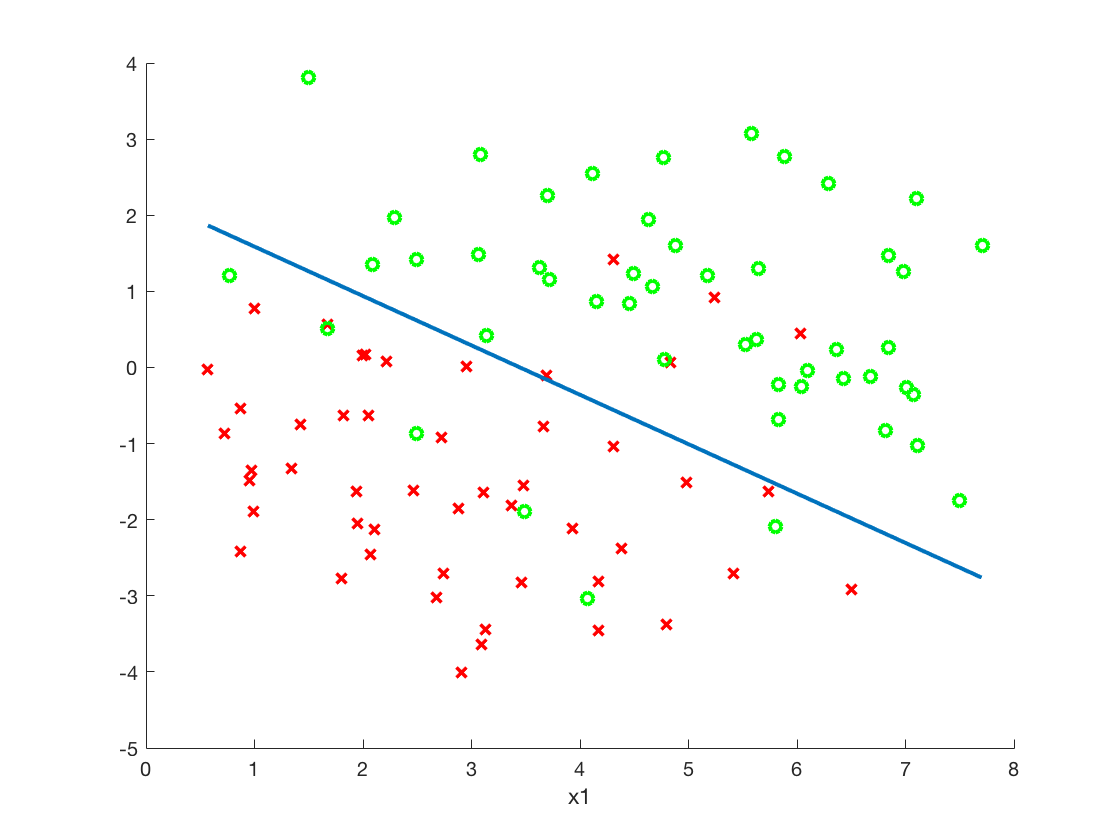
\includegraphics[width=6.5in]{ps1_1c}
\caption{The green dots are where $y^{(i)}=1$ and the red X's are where $y^{(i)}={-1}$.}
\end{figure}
}\label{prob:1c}
%%% END SUBSECTION 3 %%%%%%%%%%%%%%%%%%%%%%%%%%%%%%%%%%%%%%
}\label{problem 1}
%%% END SECTION 1 %%%%%%%%%%%%%%%%%%%%%%%%%%%%%%%%%%%%%%%%%
\section{}{
\subsection{}{
\quad We can demonstrate that the Poisson distribution is a member of the exponential family.
\begin{align*}
	p(y;\lambda) &= \frac{e^{-\lambda}\lambda^y}{y!}
    \\&=\frac{1}{y!} \exp(\log e^{-\lambda}\lambda^y)
    \\&=\frac{1}{y!} \exp(y\log\lambda - \lambda)
\end{align*}
Thus, $b(y)=\frac{1}{y!}$, $T(y)=y$, $\eta=\log\lambda$, and $a(\eta)=\lambda$.
}\label{prob:2a}
%%% END SUBSECTION 1 %%%%%%%%%%%%%%%%%%%%%%%%%%%%%%%%%%%%%%
\subsection{}{
\quad Since the Poisson distribution is in the exponential family, we can perform regression using GLM with it.
\begin{align*}
	h_\theta(x)&=E[y|x;\theta]
    \\&= \lambda
    \\&= e^\eta
    \\&= e^{\theta^Tx}
\end{align*}
Thus, the canonical response function of the Poisson distribution is $h(x) = e^\eta = e^{\theta^Tx}$.
}\label{prob:2b}
%%% END SUBSECTION 2 %%%%%%%%%%%%%%%%%%%%%%%%%%%%%%%%%%%%%%
\subsection{}{
\quad Given a training set $\{(x^{(i)}, y^{(i)});i=1\ldots m\}$, we can calculate the stochastic gradient ascent for a GLM with Poisson response $y$ and the canonical response function $h(x)$. 
\quad First, we calculate the conditional probability
\begin{align*}
	p(y^{(i)}|x^{(i)};\theta) &= \frac{1}{y^{(i)}!} \exp(y^{(i)}\theta^Tx^{(i)}-e^{\theta^Tx^{(i)}}).
\end{align*}
Then, we can calculate the derivative of the log-likelihood with respect to $\theta_j$.
\begin{align*}
	\pdv{}{\theta_j} \ell(\theta) &= \sum_{i=1}^{n} \log(\frac{1}{y^{(i)}} \exp(y^{(i)}\theta^Tx^{(i)} - e^{\theta^Tx^{(i)}}))
    \\&= \sum_{i=1}^n y^{(i)}x^{(i)}_j - x^{(i)}_je^{\theta^Tx^{(i)}}
\end{align*}
Thus, the stochastic gradient ascent update rule for a GLM with a Poisson response would be $\theta_j \coloneqq \theta_j - \alpha(h(x)-y)x_j$
}\label{prob:2c}
%%% END SUBSECTION 3 %%%%%%%%%%%%%%%%%%%%%%%%%%%%%%%%%%%%%%
\subsection{}{
\begin{proof}
\quad Given a GLM with a response variable from any of the exponential family in which $T(y) = y$ and a canonical response $h(x)$, we have that $p(y;\eta) = b(y)\exp(\eta^TT(y)-a(\eta))$, where $a(x)=h(x)$ due to the moment property of exponential family. First, we let $\eta_i=\theta^Tx_i$ and calculate the derivative of the log-likelihood with respect to $\theta_i$.
\begin{align*}
	\pdv{}{\theta_i} \ell(y|x;\theta) &= \pdv{}{\theta_i} y\theta^Tx - a(\theta^Tx) + \log(b(y))
    \\&= yx_i - \pdv{a(\theta^Tx)}{\theta_i}
    \\&= yx_i - h(x)x_i
\end{align*}
Thus, the stochastic gradient ascent update rule would be $\theta_i \coloneqq \theta_i -\alpha(h(x) - y)x_i$.
\end{proof}
}\label{prob:2d}
%%% END SUBSECTION 4 %%%%%%%%%%%%%%%%%%%%%%%%%%%%%%%%%%%%%%
}\label{problem 2}
%%% END SECTION 2 %%%%%%%%%%%%%%%%%%%%%%%%%%%%%%%%%%%%%%%%%

\section{}{
\subsection{}{
\quad We consider the case $y=1$ to calculate the posterior. Given the Bernoulli likelihood and multivariate Gaussian prior, we can calculate the posterior as follows.
\begin{align*}
	p(y|x;\phi,\Sigma, \mu_{1}, \mu_{-1}) &= \frac{p(x|y)p(y)}{p(x)}
    \\&=\frac{p(x|y=1)p(y)}{p(x|y=1)p(y=1)+p(x|y=-1)p(y=-1)}
\end{align*}
To simplify the algebra, we let $\sigma = \frac{1}{(2\pi)^{n/2}|\Sigma|^{1/2}}$ and $\mu_{y}' = \frac{-1}{2}(x-\mu_y)^T\Sigma^{-1}(x-\mu_y)$.
\begin{align*}
	p(y|x;\phi,\Sigma, \mu_{1}, \mu_{-1}) &= \frac{\sigma e^{\mu_1} \phi}{\sigma e^{\mu_1} \phi + \sigma e^{\mu_{-1}} (1-\phi)}
    \\&= \frac{1}{1+\frac{1-\phi}{\phi} e^{\mu_{-1} - \mu_1}}
    \\&= \frac{1}{1 + \exp(\log\frac{1-\phi}{\phi} - \frac{1}{2}(x-\mu_{-1})^T) \Sigma^{-1} (x-\mu_{-1}) + \frac{1}{2}(x-\mu_1)^T\Sigma^{-1}(x-\mu_1)}
    \\&= \frac{1}{1+ \exp(\log\frac{1-\phi}{\phi} + \frac{1}{2}\mu_1^T\Sigma^{-1}\mu_1-\frac{1}{2}\mu_{-1}^T\Sigma^{-1}\mu_{-1} + (\mu_{-1}-\mu_1)^T\Sigma^{-1}x)}
    \\&=\frac{1}{1+\exp(-y(\theta^Tx+\theta_0))}
\end{align*}
where $\theta^T = (\mu_{-1}-\mu_1)^T\Sigma^{-1}x$ and $\theta_0 = \log\frac{1-\phi}{\phi} + \frac{1}{2}\mu_1^T\Sigma^{-1}\mu_1-\frac{1}{2}\mu_{-1}^T\Sigma^{-1}\mu_{-1}$.
}\label{prob:3a}
%%% END SUBSECTION 1 %%%%%%%%%%%%%%%%%%%%%%%%%%%%%%%%%%%%%%%%%
\subsection{}{
\quad See \ref{prob:3c} but reduced down to one dimension.
}\label{prob:3b}
%%% END SUBSECTION 2 %%%%%%%%%%%%%%%%%%%%%%%%%%%%%%%%%%%%%%%%%
\subsection{}{
\quad We can calculate the maximum likelihood estimates given the log-likelihood
\begin{align*}
	\ell(\phi,\Sigma, \mu_{1}, \mu_{-1}) &= \log\prod_{i=1}^m p(x^{(i)}|y^{(i)}; \Sigma, \mu_{1}, \mu_{-1})p(y^{(i)};\phi)
    \\&= \sum_{i=1}^m\log p(x^{(i)}|y=y^{(i)}; \Sigma, \mu_{1}, \mu_{-1}) + \log p(y^{(i)};\phi)
    \\&= \sum_{i=1}^m -\log((2\pi)^{n/2}|\Sigma|^{1/2}) + \frac{-1}{2}(x^{(i)}-\mu_{y^{(i)}})^T \Sigma^{-1} (x^{(i)}-\mu_{y^{(i)}}) 
    \\&\hphantom{\sum_{i=1}^m-} + 1\{y^{(i)} = 1\}\log\phi + (1-1\{y^{(i)} = 1\}) \log(1-\phi)
\end{align*}
\quad To determine the maximum likelihood of each parameter, we take the derivative of each parameter individually and set the derivative equal to zero as follows.
\begin{align*}
	\pdv{\ell(\phi,\Sigma, \mu_{1}, \mu_{-1})}{\phi} &= 0
    \\ \sum_{i=1}^m \frac{1\{y^{(i)} = 1\}}{\phi} - \frac{1-1\{y^{(i)} = 1\}}{1-\phi} &= 0
    \\ \sum_{i=1}^m \frac{1\{y^{(i)} = 1\}}{\phi} &= \sum_{i=1}^m \frac{1-1\{y^{(i)} = 1\}}{1-\phi}
    \\ (1-\phi)\sum_{i=1}^m 1\{y^{(i)} = 1\} &= \phi\sum_{i=1}^m 1-1\{y^{(i)} = 1\}
    \\ \sum_{i=1}^m 1\{y^{(i)} = 1\} - \phi\sum_{i=1}^m 1\{y^{(i)} = 1\} &= m\phi - \phi \sum_{i=1}^m 1\{y^{(i)} = 1\}
    \\ \phi &= \frac{1}{m} \sum_{i=1}^m 1\{y^{(i)} = 1\}
\end{align*}
Thus, the maximum likelihood for $\phi$ is given by $\phi = \frac{1}{m} \sum_{i=1}^m \{y^{(i)} = 1\}$.
\begin{align*}
	\pdv{\ell(\phi,\Sigma, \mu_{1}, \mu_{-1})}{\mu_{y^{(i)}}} &= 0
    \\ \sum_{i=1}^m \frac{-1}{2} (-\Sigma^{-1}x^{(i)} - \Sigma^{-1}x^{(i)} + \Sigma^{-1}\mu_{y^{(i)}} + \Sigma^{-1}\mu_{y^{(i)}}) 1\{y^{(i)} = 1\}&= 0
    \\ \sum_{i=1}^m (\Sigma^{-1}x^{(i)} - \Sigma^{-1}\mu_{y^{(i)}}) 1\{y^{(i)} = 1\}&= 0
    \\ \sum_{i=1}^m (\Sigma^{-1}x^{(i)}) 1\{y^{(i)} = 1\} &= \sum_{i=1}^m (\Sigma^{-1}\mu_{y^{(i)}}) 1\{y^{(i)} = 1\}
    \\ \mu_{y^{(i)}} &= \frac{\sum_{i=1}^m x^{(i)} 1\{y^{(i)} = 1\}}{\sum_{i=1}^m 1\{y^{(i)} = 1\}}
\end{align*}
Thus, the maximum likelihood for $\mu_{y^{(i)}}$ is given by $\mu_{y^{(i)}} = \frac{\sum_{i=1}^m x^{(i)} 1\{y^{(i)} = 1\}}{\sum_{i=1}^m 1\{y^{(i)} = 1\}}$.
\\ \quad To calculate the maximum likelihood for $\Sigma$, we let $S=\Sigma^{-1}$ to simplify the algebra.
\begin{align*}
	\pdv{\ell(\phi,\Sigma, \mu_{1}, \mu_{-1})}{S} &= 0
    \\ \sum_{i=1}^m  \frac{(2\pi)^{n/2}}{|S^{-1}|^{1/2}} \frac{1}{2(2\pi)^{n/2}|S^{-1}|^{1/2}} \nabla_S|S| \hphantom{(x^{(i)}-\mu_{y^{(i)}})} &
    \\- \nabla_S \frac{-1}{2}(x^{(i)}-\mu_{y^{(i)}})^T S (x^{(i)}-\mu_{y^{(i)}}) &= 0
    \\ \sum_{i=1}^m \frac{1}{2} (S^{-1})^T - \frac{-1}{2}(x^{(i)}-\mu_{y^{(i)}})^T (x^{(i)}-\mu_{y^{(i)}}) &= 0
    \\ (S^{-1})^T m &= \sum_{i=1}^m (x^{(i)}-\mu_{y^{(i)}})^T (x^{(i)}-\mu_{y^{(i)}})
    \\ \Sigma &= \frac{1}{m} \sum_{i=1}^m (x^{(i)}-\mu_{y^{(i)}})^T (x^{(i)}-\mu_{y^{(i)}})
\end{align*}
Thus, the maximum likelihood for $\Sigma$ is $\Sigma = \frac{1}{m} \sum_{i=1}^m (x^{(i)}-\mu_{y^{(i)}})^T (x^{(i)}-\mu_{y^{(i)}})$.
}\label{prob:3c}
%%% END SUBSECTION 3 %%%%%%%%%%%%%%%%%%%%%%%%%%%%%%%%%%%%%%%%%
}\label{problem 3}
%%% END SECTION 3 %%%%%%%%%%%%%%%%%%%%%%%%%%%%%%%%%%%%%%%%%

\section{}{
\subsection{}{
\begin{proof}
Given a matrix $A\in\R^{n\times n}$, vectors $x, z \in\R^n$, where $x = Az$ and $x^{(0)} = \vec{0}$, and the function $g(z) = f(Az)$, we first need to find the gradient and Hessian of $g(z)$.
\begin{align*}
	\nabla g(z) &= \sum_{i} \pdv{g(z)}{z_i}
    \\&= \sum_{i} \pdv{f(Az)}{z_i}
    \\&= \sum_{i} A_i \nabla f(Az)
    \\&= A^T \nabla f(Az)
\end{align*}
Thus, $\nabla g(z) = A^T \nabla f(Az)$.
\begin{align*}
	\nabla^2g(z) &= \sum_{i}\sum{j} \pdv{g(z)}{z_i}{z_j}
    \\&= \sum_{i}\sum{j} \pdv{f(Az)}{z_i}{z_j}
    \\&= \sum_{i}\sum{j} \pdv{}{z_j} A_i \nabla f(Az)
    \\&= \sum_{i}\sum{j} A_iA_j \nabla^2 f(Az)
    \\&= A^TA \nabla^2 f(Az)
\end{align*}
Thus, $\nabla^2 g(z) = A^TA \nabla^2 f(Az)$.
\\ \quad We can now show that Newton's method is invariant to linear reparametrization as follows.
\begin{align*}
	z^{(i+1)} &\coloneqq z^{(i)} - (\nabla^2 g(z^{(i)}))^{-1} \bullet (\nabla g(z^{(i)}))
    \\&= z^{(i)} - (A^TA\nabla^2 f(Az^{(i)}))^{-1} \bullet (A^T \nabla f(Az^{(i)}))
    \\&= z^{(i)} - A^{-1}(\nabla^2 f(Az^{(i)}))^{-1} \bullet (\nabla f(Az^{(i)}))
  \\Az^{(i+1)} &\coloneqq Az^{(i)} - (\nabla^2 f(Az^{(i)}))^{-1} \bullet (\nabla f(Az^{(i)}))
  \\x^{(i+1)} &\coloneqq x^{(i)} - (\nabla^2 f(x^{(i)}))^{-1} \bullet (\nabla f(x^{(i)}))
\end{align*}
Since, when $x^{(i)} = Az^{(i)}$, $x^{(i+1)} = Az^{(i+1)}$ and it is obvious that $x^{(0)} = \vec{0} = z^{(0)}$, Newton's method is invariant to linear reparametrization.
\end{proof}
}\label{prob:4a}
%%% END SUBSECTION 1 %%%%%%%%%%%%%%%%%%%%%%%%%%%%%%%%%%%%%%%%%%%%
\subsection{}{
Using the same assumptions as in problem \ref{prob:4a}, we can show that gradient descent is not invariant to linear reparamtarization.
\begin{align*}
	z^{(i+1)} &\coloneqq z^{(i)} - \alpha \nabla g(z^{(i)})
    \\&= z^{(i)} - \alpha A^T \nabla f(Az^{(i)})
  \\(A^T)^{-1}z^{(i+1)} &\coloneqq (A^T)^{-1} z^{(i)} - \alpha f(Az^{(i)})
\end{align*}
Since it is obvious that $x^{(i+1)} \neq (A^T)^{-1}z^{(i+1)}$, we are at an impasse. Thus, gradient descent is not invariant to linear reparametrization.
}\label{prob:4b}
%%% END SUBSECTION 2 %%%%%%%%%%%%%%%%%%%%%%%%%%%%%%%%%%%%%%%%%%%%
}\label{problem 4}
%%% END SECTION 4 %%%%%%%%%%%%%%%%%%%%%%%%%%%%%%%%%%%%%%%%%

\section{}{
\subsection*{Part a}{
\subsubsection*{5.a.i}{%
\quad Given that $X$, the matrix of input vectors, $\vec{y}$, the output vector, and $W$ is a diagonal matrix with the diagonal elements are $\frac{1}{2} w^{(i)}$, where $w^{(i)}$ is the weight of the $i$-th element, are the proper dimensions, 
\begin{align*}
	J(\theta) &= (X\theta - \vec{y})^TW(X\theta - \vec{y})
    \\&= \sum_i (x^{(i)}\theta-y^{(i)})^2\frac{1}{2}w_{ii}
    \\&= \frac{1}{2} \sum_i w^{(i)}(\theta^Tx^{(i)}-y^{(i)})^2
\end{align*}
Thus, $(X\theta - \vec{y})^TW(X\theta - \vec{y}) = \frac{1}{2} \sum_i w^{(i)}(\theta^Tx^{(i)}-y^{(i)})^2$.
}\label{prob:5a1}
%%% END SUBSUBSECTION 1 %%%%%%%%%%%%%%%%%%%%%%%%%%%%%%%%%%%%%%%%%%%%%%%%%%
\subsubsection*{5.a.ii}{
We can also extend the normal equation to include the weight matrix $W$.
\begin{align*}
	\\ \pdv{J(\theta)}{\theta} &= 0
	\\ \pdv{\theta} (X\theta - \vec{y})^TW(X\theta - \vec{y}) &= 0
    \\ X^TWX\theta + (\theta^TX^TWX)^T - X^TWy^T - (yWX)^T &= 0
    \\ X^TWX\theta + X^TWX\theta - X^TWy^T - X^TWy^T &= 0
  \\X^TWX\theta &= X^TWy^T
  \\ \theta &= (X^TWX)^{-1}X^TWy^T
\end{align*}
Thus, the normal equation including the weights is $\theta = (X^TWX)^{-1}X^TWy^T$.
}\label{prob:5a2}
%%% END SUBSUBSECTION 2 %%%%%%%%%%%%%%%%%%%%%%%%%%%%%%%%%%%%%%%%%%%%%%%%%%
\subsubsection*{5.a.ii}{
For the training set $\{(x^{(i)},y^{(i)});i=1,\ldots,m\}$ and given that 
\begin{align*}
	p(y^{(i)}|x^{(i)};\theta) &= \frac{1}{\sqrt[]{2\pi}\sigma^{(i)}} \exp(-\frac{(y^{(i)}-\theta^Tx^{(i)})^2}{2(\sigma^{(i)})^2}),
\end{align*}
the maximum likelihood is simply solving a weighted linear regression as follows.
\begin{align*}
	\arg\max_\theta \ell(\theta) &= \log \prod_{i=1}^m p(y^{(i)}|x^{(i)};\theta)
    \\&= \sum_{i=1}^m \log \frac{1}{\sqrt[]{2\pi}\sigma^{(i)}} - \frac{(y^{(i)}-\theta^Tx^{(i)})^2}{2(\sigma^{(i)})^2}
    \\&= \sum_{i=1}^m \frac{-1}{2(\sigma^{(i)})^2} (y^{(i)}-\theta^Tx^{(i)})^2
  \\ \arg \min_\theta \ell(\theta) &= \frac{1}{2} \sum_{i=1}^m \frac{1}{\sigma^2} (y^{(i)}-\theta^Tx^{(i)})^2
\end{align*}
Thus, fitting $\theta$ for a normally distributed set is essentially solving a weighted linear regression with $w^{(i)} = \frac{1}{(\sigma^{(i)})^2}$.
}\label{prob:5a3}
%%% END SUBSUBSECTION 3 %%%%%%%%%%%%%%%%%%%%%%%%%%%%%%%%%%%%%%%%%%%%%%%%%%
}\label{prob:5a}
%%% END SUBSECTION 1 %%%%%%%%%%%%%%%%%%%%%%%%%%%%%%%%%%%%%%%%%%%%
\subsection*{Part b}{
\subsubsection*{5.b.i}{
We can fit an unweighted least squares regression to the first training example using the following code.
\begin{lstlisting}
% Load in data
run('load_quasar_data.m');

% Non-weighted model fitted with the first training example
X = lambdas;
Y = train_qso(1,:)';
theta = inv(X' * X) * X' * Y;

% Plot non-weighted model and corresponding points
figure; hold on;
plot(X, Y, 'go', 'linewidth', 2);
x1 = min(X):1:max(X);
x2 = theta * x1;
plot(x1, x2, 'linewidth', 2);
xlabel('lambda');
ylabel('flux');
\end{lstlisting}
With this code, we get the following plot.
\begin{figure}[h]
\centering
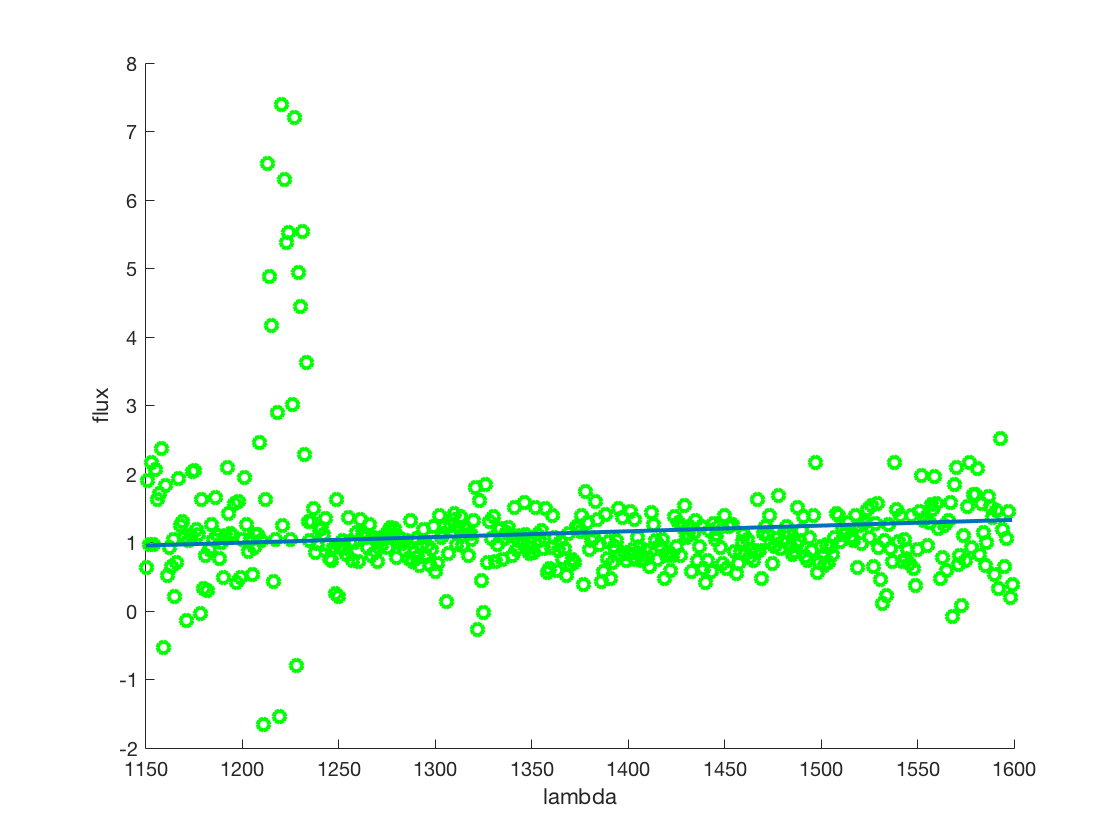
\includegraphics[width=6.5in]{ps1_5b1}
\caption{The green dots are where the true values and the line is the predicted values.}
\end{figure}
}\label{prob:5b1}
%%% END SUBSUBSECTION 1 %%%%%%%%%%%%%%%%%%%%%%%%%%%%%%%%%%%%%%%%%%%%%%%%%%
\subsubsection*{5.b.ii}{
We can also fit a weighted least squares regression to the first training example using the following code.
\begin{lstlisting}
% Load in data
run('load_quasar_data.m');

% Weighted model fitted with the first training example
X = lambdas;
Y = train_qso(1,:)';
taus = [5];

% Make plot for weighted model
figure; hold on;
plot(lambdas, Y, 'kx', 'linewidth', 2);
x1 = min(lambdas):1:max(lambdas);
xlabel('lambda');
ylabel('flux');

% Fit weighted model for each value of tau
for tau = taus   
    y = [];
    for xi = lambdas'
        w = exp(-(xi - X).^2/(2*tau^2));
        W = diag(w, 0);
        theta = inv(X' * W * X) * X' * W * Y;
        y = [y theta*xi];
    end
x2 = y';
plot(x1, x2, 'linewidth', 2);
end
\end{lstlisting}
With this code, we get the following plot.
\begin{figure}[H]
\centering
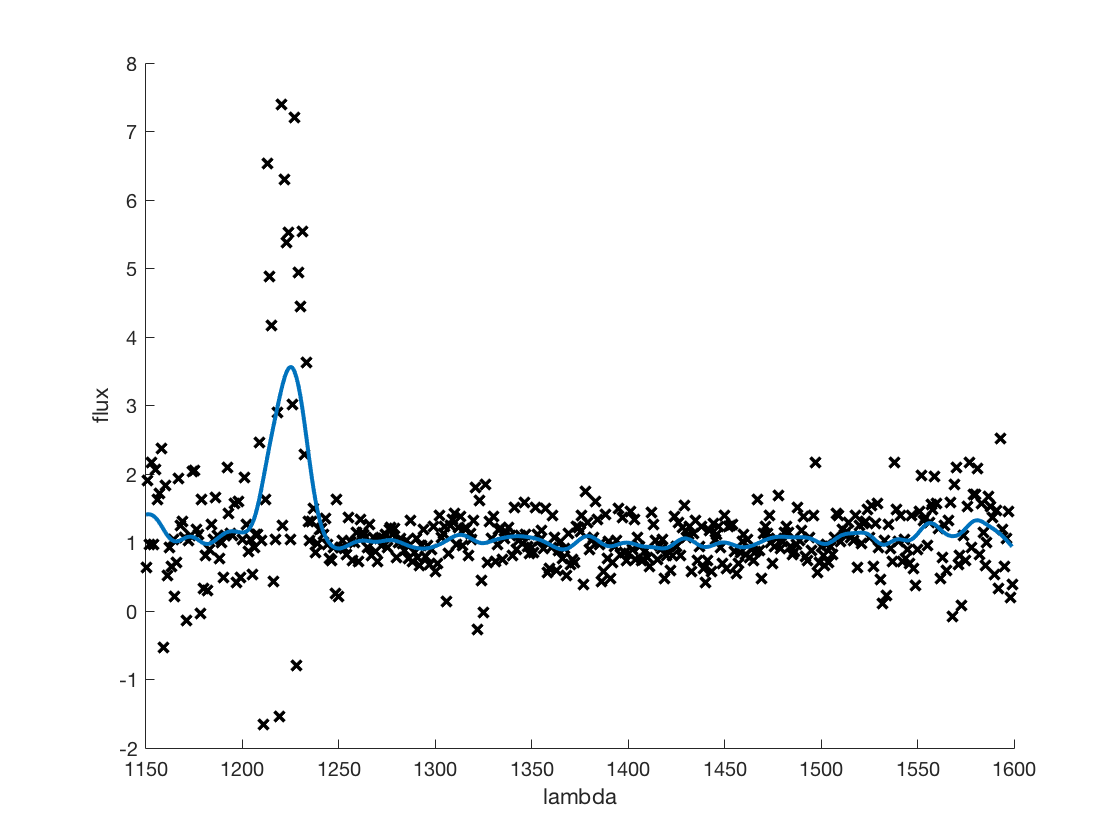
\includegraphics[width=6.5in]{ps1_5b2}
\caption{The black x's are where the true values and the line is the predicted values.}
\end{figure}
}\label{prob:5b2}
%%% END SUBSUBSECTION 2 %%%%%%%%%%%%%%%%%%%%%%%%%%%%%%%%%%%%%%%%%%%%%%%%%%
\subsubsection*{5.b.iii}{
We can also modify the code to be the following to explore the effect of $\tau$.
\begin{lstlisting}
% Load in data
run('load_quasar_data.m');

% Weighted model fitted with the first training example
X = lambdas;
Y = train_qso(1,:)';
% taus = [5];
taus = [1, 10, 100, 1000];

% Make plot for weighted model
figure; hold on;
plot(lambdas, Y, 'kx', 'linewidth', 2);
x1 = min(lambdas):1:max(lambdas);
xlabel('lambda');
ylabel('flux');

% Fit weighted model for each value of tau
for tau = taus   
    y = [];
    for xi = lambdas'
        w = exp(-(xi - X).^2/(2*tau^2));
        W = diag(w, 0);
        theta = inv(X' * W * X) * X' * W * Y;
        y = [y theta*xi];
    end
x2 = y';
plot(x1, x2, 'linewidth', 2);
end
\end{lstlisting}
With this code, we get the following plot.
\begin{figure}[H]
\centering
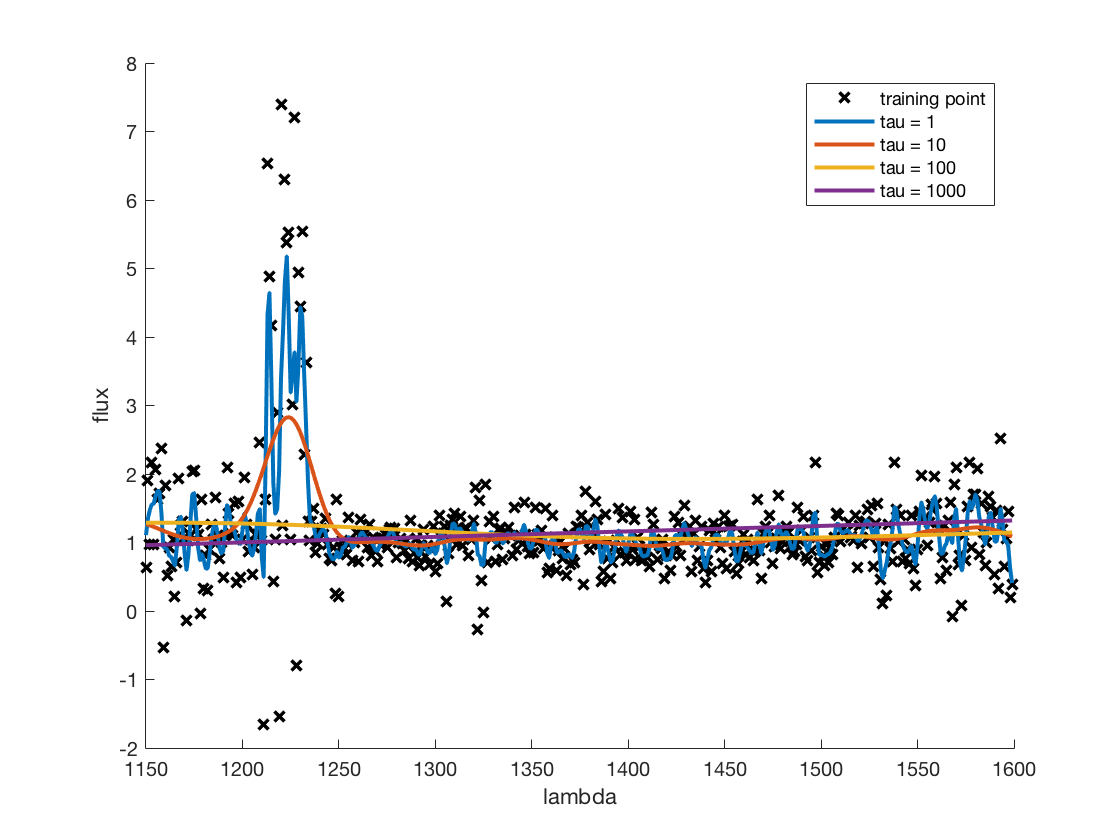
\includegraphics[width=6.5in]{ps1_5b3}
\caption{The black x's are where the true values and the lines are the different predicted values correlating to different values of $\tau$.}
\end{figure}
We notice that the larger the value of $\tau$, the "smoother" the line becomes. This is due to the fact that larger values of $\tau$ reduce the weight of points. Thus, the larger the $\tau$ the smaller effect the weights will have.
}\label{prob:5b3}
%%% END SUBSUBSECTION 3 %%%%%%%%%%%%%%%%%%%%%%%%%%%%%%%%%%%%%%%%%%%%%%%%%%
}\label{prob:5b}
%%% END SUBSECTION 2 %%%%%%%%%%%%%%%%%%%%%%%%%%%%%%%%%%%%%%%%%%%%
}\label{problem 5}
%%% END SECTION 5 %%%%%%%%%%%%%%%%%%%%%%%%%%%%%%%%%%%%%%%%%
\end{document}